
\SetKwFunction{FDPTimelines}{DPTimelines}
\begin{figure}[htp]
    \begin{minipage}[t]{0.17\textwidth}
    \centering
    \begin{tikzpicture}[every node/.style={draw, very thick, drop shadow}, every path/.style={very thick}]
    
    \node[circle, draw, minimum size=0.35cm, inner sep=0pt, fill=white] (1) at (0,0) {};

    \node[circle, draw, minimum size=0.35cm, inner sep=0pt, fill=black] (2) at (-0.2,-0.8) {};

    \node[circle, draw, minimum size=0.35cm, inner sep=0pt, fill=white] (3) at (-0.4,-1.6) {};

    \node[circle, draw, minimum size=0.35cm, inner sep=0pt, fill=white] (4) at (-0.6,-2.4) {};

    \node[circle, draw, minimum size=0.35cm, inner sep=0pt, fill=white] (5) at (-0.8,-3.2) {};

    \node[circle, draw, minimum size=0.35cm, inner sep=0pt, fill=black] (6) at (-1,-4) {};

    \node[circle, draw, minimum size=0.35cm, inner sep=0pt, fill=white] (7) at (-1.2,-4.8) {};


    \draw[] (1) to (2);

    \draw[] (2) to (3);

    \draw[] (3) to (4);
    
    \draw[] (4) to (5);
    
    \draw[] (5) to (6);
    
    \draw[] (6) to (7);
    \end{tikzpicture}
    \caption[Timeline $P$]{}\label{timeline}
\end{minipage}
\begin{minipage}[t]{0.27\textwidth}
    \centering
    \begin{tikzpicture}[every node/.style={draw, very thick, drop shadow}, every path/.style={very thick}]
    
    \node[circle, draw, minimum size=0.35cm, inner sep=0pt, fill=white] (1) at (-1.4,0) {};

    \node[circle, draw, minimum size=0.35cm, inner sep=0pt, fill=black] (2) at (-1.6,-0.8) {};

    \node[circle, draw, minimum size=0.35cm, inner sep=0pt, fill=black] (3) at (-1.8,-1.6) {};

    \node[circle, draw, minimum size=0.35cm, inner sep=0pt, fill=white] (4) at (-2,-2.4) {};

    \node[circle, draw, minimum size=0.35cm, inner sep=0pt, fill=black] (5) at (-2.2,-3.2) {};

    \node[circle, draw, minimum size=0.35cm, inner sep=0pt, fill=black] (6) at (-2.4,-4) {};

    \node[circle, draw, minimum size=0.35cm, inner sep=0pt, fill=white] (7) at (-2.6,-4.8) {};


    \draw[] (1) to (2);

    \draw[] (2) to (3);

    \draw[] (3) to (4);
    
    \draw[] (4) to (5);
    
    \draw[] (5) to (6);
    
    \draw[] (6) to (7);
    
    \node[circle, draw, minimum size=0.35cm, inner sep=0pt, fill=black] (11) at (-0,0) {};

    \node[circle, draw, minimum size=0.35cm, inner sep=0pt, fill=black] (12) at (-0.2,-0.8) {};

    \node[circle, draw, minimum size=0.35cm, inner sep=0pt, fill=white] (13) at (-0.4,-1.6) {};

    \node[circle, draw, minimum size=0.35cm, inner sep=0pt, fill=black] (14) at (-0.6,-2.4) {};

    \node[circle, draw, minimum size=0.35cm, inner sep=0pt, fill=white] (15) at (-0.8,-3.2) {};

    \node[circle, draw, minimum size=0.35cm, inner sep=0pt, fill=black] (16) at (-1,-4) {};

    \node[circle, draw, minimum size=0.35cm, inner sep=0pt, fill=black] (17) at (-1.2,-4.8) {};


    \draw[] (11) to (12);

    \draw[] (12) to (13);

    \draw[] (13) to (14);
    
    \draw[] (14) to (15);
    
    \draw[] (15) to (16);
    
    \draw[] (16) to (17);
    \end{tikzpicture}
    \caption[Bipartition $\br{I_1, I_2}$]{}\label{bipartition}
\end{minipage}
\begin{minipage}[t]{0.37\textwidth}
    \centering
    \begin{tikzpicture}[every path/.style={very thick}]
    
    \node[circle, draw, minimum size=0.35cm, inner sep=0pt, fill=white] (1) at (-1.4,0) {};

    \node[circle, draw, minimum size=0.35cm, inner sep=0pt, fill=black] (2) at (-1.6,-0.8) {};

    \node[circle, draw, minimum size=0.35cm, inner sep=0pt, fill=black] (3) at (-1.8,-1.6) {};

    \node[circle, draw, minimum size=0.35cm, inner sep=0pt, fill=white] (4) at (-2,-2.4) {$v$};

    \node[circle, draw, minimum size=0.35cm, inner sep=0pt, fill=black] (5) at (-2.2,-3.2) {};

    \node[circle, draw, minimum size=0.35cm, inner sep=0pt, fill=black] (6) at (-2.4,-4) {};

    \node[circle, draw, minimum size=0.35cm, inner sep=0pt, fill=white] (7) at (-2.6,-4.8) {};

    \draw[] (1) to (2);

    \draw[] (2) to (3);

    \draw[] (3) to (4);
    
    \draw[] (4) to (5);
    
    \draw[] (5) to (6);
    
    \draw[] (6) to (7);

    \draw[very thick, fill=gray!20, drop shadow] (-0.8,-1) -- (-1.1,-1.6) -- (-0.5,-1.6) -- cycle;

    \draw[very thick, fill=gray!20, drop shadow] (0.2,-0.9) -- (0.6,-1.7) -- (-0.2,-1.7) -- cycle;


    \node at (0.85, -1.25) {$\dots$}; 

    \draw[very thick, fill=gray!20, drop shadow] (1.5,-0.8) -- (1,-1.8) -- (2,-1.8) -- cycle;

    \draw[very thick] (1) -- (-0.8,-1);
    \draw[very thick] (1) -- (0.2,-0.9);
    \draw[very thick] (1) -- (1.5,-0.8);

    \draw[very thick, fill=gray!20, drop shadow] (-1.2,-3.3) -- (-1.8,-4.5) -- (-0.6,-4.5) -- cycle;

    \draw[very thick, fill=gray!20, drop shadow] (0.4,-3.2) -- (-0.3,-4.6) -- (1.1,-4.6) -- cycle;

    \draw[very thick] (4) -- (-1.2,-3.3);
    
    \draw[very thick] (4) -- (0.4,-3.2);

    \end{tikzpicture}
    \caption[Decision Tree $D_1$]{}\label{D1}
\end{minipage}
\begin{minipage}[t]{0.15\textwidth}
    \centering
    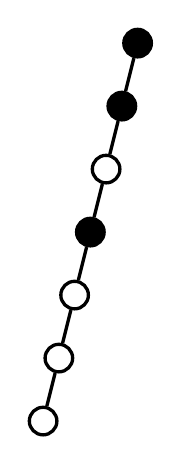
\begin{tikzpicture}[every path/.style={very thick}]
    
    \node[circle, draw, minimum size=0.35cm, inner sep=0pt, fill=black] (11) at (-0,0) {};

    \node[circle, draw, minimum size=0.35cm, inner sep=0pt, fill=black] (12) at (-0.2,-0.8) {};

    \node[circle, draw, minimum size=0.35cm, inner sep=0pt, fill=white] (13) at (-0.4,-1.6) {};

    \node[circle, draw, minimum size=0.35cm, inner sep=0pt, fill=black] (14) at (-0.6,-2.4) {};

    \node[circle, draw, minimum size=0.35cm, inner sep=0pt, fill=white] (15) at (-0.8,-3.2) {};

    \node[circle, draw, minimum size=0.35cm, inner sep=0pt, fill=white] (16) at (-1,-4) {};

    \node[circle, draw, minimum size=0.35cm, inner sep=0pt, fill=white] (17) at (-1.2,-4.8) {};


    \draw[] (11) to (12);

    \draw[] (12) to (13);

    \draw[] (13) to (14);
    
    \draw[] (14) to (15);
    
    \draw[] (15) to (16);
    
    \draw[] (16) to (17);

    \end{tikzpicture}
    \caption[Timeline $P_2$]{}\label{P2}
\end{minipage}

\begin{minipage}[t]{0.3\textwidth}
    \centering
    \begin{tikzpicture}[every path/.style={very thick}]
    
    \node[circle, draw, minimum size=0.35cm, inner sep=0pt, fill=black] (11) at (-0,0) {};

    \node[circle, draw, minimum size=0.35cm, inner sep=0pt, fill=black] (12) at (-0.2,-0.8) {};

    \node[circle, draw, minimum size=0.35cm, inner sep=0pt, fill=white] (13) at (-0.4,-1.6) {};

    \node[circle, draw, minimum size=0.35cm, inner sep=0pt, fill=black] (14) at (-0.6,-2.4) {};

    \node[circle, draw, minimum size=0.35cm, inner sep=0pt, fill=white] (15) at (-0.8,-3.2) {};

    \node[circle, draw, minimum size=0.35cm, inner sep=0pt, fill=white] (16) at (-1,-4) {};

    \node[circle, draw, minimum size=0.35cm, inner sep=0pt, fill=white] (17) at (-1.2,-4.8) {};


    \draw[] (11) to (12);

    \draw[] (12) to (13);

    \draw[] (13) to (14);
    
    \draw[] (14) to (15);
    
    \draw[] (15) to (16);
    
    \draw[] (16) to (17);
    
    \draw[very thick, fill=white, drop shadow] (0.3,-2.5) -- (0.7,-3.3) -- (-0.1,-3.3) -- cycle;

    \draw[very thick, fill=white, drop shadow] (1.5,-2.4) -- (1,-3.4) -- (2,-3.4) -- cycle;

    \draw[very thick] (13) -- (0.3,-2.5);
    
    \draw[very thick] (13) -- (1.5,-2.4);

    \draw[very thick, fill=white, drop shadow] (0.6,-4) -- (0.1,-5) -- (1.1,-5) -- cycle;

    \draw[very thick] (15) -- (0.6,-4);

    \draw[very thick, fill=white, drop shadow] (-0.4,-4.3) -- (-0.1,-4.9) -- (-0.7,-4.9) -- cycle;

    \draw[very thick] (16) -- (-0.4,-4.3);

    \end{tikzpicture}
    \caption[Decision tree $D_2$]{}\label{D2}
\end{minipage}
\begin{minipage}[t]{0.3\textwidth}
    \centering
    \begin{tikzpicture}[every path/.style={very thick}]
    
    \node[circle, draw, minimum size=0.35cm, inner sep=0pt, fill=black] (11) at (-0,0) {};

    \node[circle, draw, minimum size=0.35cm, inner sep=0pt, fill=black] (12) at (-0.2,-0.8) {};

    \node[circle, draw, minimum size=0.35cm, inner sep=0pt, fill=white] (13) at (-0.4,-1.6) {};

    \node[circle, draw, minimum size=0.35cm, inner sep=0pt, fill=black] (14) at (-0.6,-2.4) {};

    \node[circle, draw, minimum size=0.35cm, inner sep=0pt, fill=white] (15) at (-0.2,-3.2) {};

    \node[circle, draw, minimum size=0.35cm, inner sep=0pt, fill=white] (16) at (-0.4,-4) {};

    \node[circle, draw, minimum size=0.35cm, inner sep=0pt, fill=white] (17) at (-0.6,-4.8) {};


    \draw[] (11) to (12);

    \draw[] (12) to (13);

    \draw[] (13) to (14);
    
    \draw[] (14) to (15);
    
    \draw[] (15) to (16);
    
    \draw[] (16) to (17);
    
    \draw[very thick, fill=white, drop shadow] (0.8,-2.5) -- (1.2,-3.3) -- (0.4,-3.3) -- cycle;

    \draw[very thick, fill=white, drop shadow] (2,-2.4) -- (1.5,-3.4) -- (2.5,-3.4) -- cycle;

    \draw[very thick] (13) -- (0.8,-2.5);
    
    \draw[very thick] (13) -- (2,-2.4);

    \draw[very thick, fill=white, drop shadow] (1.2,-4) -- (0.7,-5) -- (1.7,-5) -- cycle;

    \draw[very thick] (15) -- (1.2,-4);

    \draw[very thick, fill=white, drop shadow] (0.2,-4.3) -- (0.5,-4.9) -- (-0.1,-4.9) -- cycle;

    \draw[very thick] (16) -- (0.2,-4.3);

    \end{tikzpicture}
    \caption[Rehanging step]{}\label{rehang}
\end{minipage}
\begin{minipage}[t]{0.4\textwidth}
    \centering
    \begin{tikzpicture}[every path/.style={very thick}]
    
    \node[circle, draw, minimum size=0.35cm, inner sep=0pt, fill=white] (1) at (-1.4,0) {};

    \node[circle, draw, minimum size=0.35cm, inner sep=0pt, fill=black] (2) at (-1.6,-0.8) {};

    \node[circle, draw, minimum size=0.35cm, inner sep=0pt, fill=white] (3) at (-1.8,-1.6) {};

    \node[circle, draw, minimum size=0.35cm, inner sep=0pt, fill=white] (4) at (-2,-2.4) {$v$};

    \node[circle, draw, minimum size=0.35cm, inner sep=0pt, fill=black] (5) at (-2.2,-3.2) {};

    \node[circle, draw, minimum size=0.35cm, inner sep=0pt, fill=black] (6) at (-2.4,-4) {};

    \node[circle, draw, minimum size=0.35cm, inner sep=0pt, fill=white] (7) at (-2.6,-4.8) {};

    \draw[] (1) to (2);

    \draw[] (2) to (3);

    \draw[] (3) to (4);
    
    \draw[] (4) to (5);
    
    \draw[] (5) to (6);
    
    \draw[] (6) to (7);

    \draw[very thick, fill=gray!20, drop shadow] (-0.8,-0.5) -- (-1.1,-1.1) -- (-0.5,-1.1) -- cycle;

    \draw[very thick, fill=gray!20, drop shadow] (0.2,-0.4) -- (0.6,-1.2) -- (-0.2,-1.2) -- cycle;


    \node at (0.85, -0.75) {$\dots$}; 

    \draw[very thick, fill=gray!20, drop shadow] (1.5,-0.3) -- (1,-1.3) -- (2,-1.3) -- cycle;

    \draw[very thick] (1) -- (-0.8,-0.5);
    \draw[very thick] (1) -- (0.2,-0.4);
    \draw[very thick] (1) -- (1.5,-0.3);

    \draw[very thick, fill=gray!20, drop shadow] (0.4,-3.3) -- (-0,-4.1) -- (0.8,-4.1) -- cycle;

    \draw[very thick, fill=gray!20, drop shadow] (1.6,-3.2) -- (1.1,-4.2) -- (2.1,-4.2) -- cycle;

    \draw[very thick] (4) -- (0.4,-3.3);
    
    \draw[very thick] (4) -- (1.6,-3.2);



    
    \node[circle, draw, minimum size=0.35cm, inner sep=0pt, fill=white] (15) at (-1.2,-3.2) {};

    \node[circle, draw, minimum size=0.35cm, inner sep=0pt, fill=white] (16) at (-1.4,-4) {};

    \node[circle, draw, minimum size=0.35cm, inner sep=0pt, fill=white] (17) at (-1.6,-4.8) {};

    \draw[very thick] (4) -- (15);
    \draw[very thick] (15) -- (16);
    \draw[very thick] (16) -- (17);

    \draw[very thick, fill=white, drop shadow] (-0.5,-1.9) -- (-0.2,-2.5) -- (-0.8,-2.5) -- cycle;

    \draw[very thick, fill=white, drop shadow] (0.4,-1.8) -- (0,-2.6) -- (0.8,-2.6) -- cycle;

    \draw[very thick] (3) -- (-0.5,-1.9);
    
    \draw[very thick] (3) -- (0.4,-1.8);
    
    \draw[very thick, fill=white, drop shadow] (-0.2,-4.2) -- (-0.55,-4.9) -- (0.15,-4.9) -- cycle;

    \draw[very thick] (15) -- (-0.2,-4.2);

    \draw[very thick, fill=white, drop shadow] (-1,-4.3) -- (-0.75,-4.8) -- (-1.25,-4.8) -- cycle;

    \draw[very thick] (16) -- (-1,-4.3);

    \end{tikzpicture}
    \caption[Resulting decision tree $D$]{}\label{D}
\end{minipage}
\caption[Basic steps of \texttt{DPTimelines} procedure]{Basic steps of the case when $i>1$. The black nodes are blocked and white are unassigned. Fig. \ref{timeline}: example timeline $P$. Fig. \ref{bipartition}: timelines $P_1$ and $P_2$ induced by bipartition $\br{I_1,I_2}$ of $I$. Fig \ref{D1}: decision tree $D_1$ compatible with timeline $P_1$. Fig \ref{P2}: timeline $P_2$ after unblocking nodes with indices below $k$. Fig \ref{D2}: a decision tree $D_2$ compatible with $P_2$. Fig \ref{rehang}: $D_2$ with left child of $q_k$ rehanged to right. Fig \ref{D}: $D_1$ and $D_2$ aligned by their left paths.}\label{dp_timelines_figure}
\end{figure}